\documentclass[Bachelorarbeit.tex]{subfiles}
\begin{document}

\chapter{Simulink Models}
\section{Simulink model to detect a face on an image}\label{sec:SimulinkFaceImage}
\begin{figure}[!h]
\centering
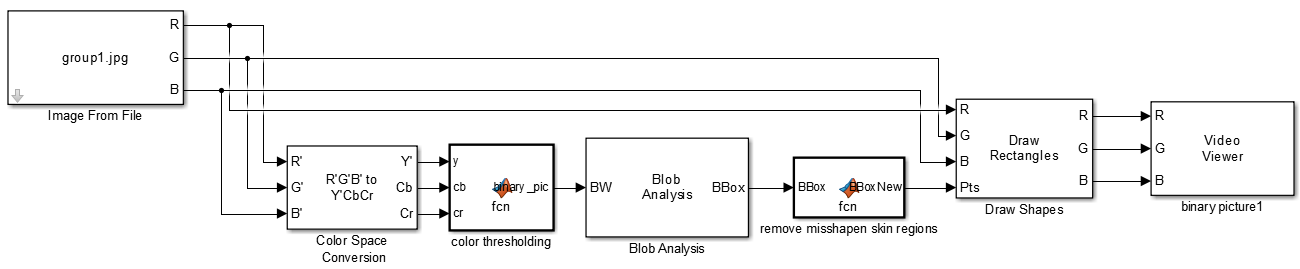
\includegraphics[width=14cm]{./img/simulink/Simulink_ImageProcessing.PNG} 
\caption{Simulink model - Face detection on an image}
\label{SimModelImage}
\end{figure}

\begin{lstlisting}[caption=MATLAB function block - color thresholding]
% University of Applied Science Vorarlberg
% Master of Mechatronics
% -------------------------------------------------------------------------
% Course: Sensor Systems
% -------------------------------------------------------------------------
% Author:       Tobias Burtscher and Stefan Stark
% Date:         10.12.2016
% Description:  Function which thresholds the YCbCr picture for face
%               detection

function binary_pic  = fcn(y,cb,cr)
    % Thresholding -> binary
    thresh_cb = cb > 76 & cb < 125;     % thresholding for cb values
    thresh_cr = cr > 140 & cr < 165;    % thresholding for cr values
    binary_pic = thresh_cb&thresh_cr;   % create binary picture

    y_th = y;                           % set output
    cb_th = cb.*(uint8(thresh_cb));     % set output cb     
    cr_th = cr.*(uint8(thresh_cr));     % set output cr
                                        % typecast is necessary to create 
                                        % a number out of the boolean
                                        % thresh_cb
end
\end{lstlisting}

\begin{lstlisting}[caption=MATLAB function block - remove misshapen skin regions]
% University of Applied Science Vorarlberg
% Master of Mechatronics
% -------------------------------------------------------------------------
% Course: Sensor Systems
% -------------------------------------------------------------------------
% Author:       Tobias Burtscher and Stefan Stark
% Date:         10.12.2016
% Description:  Function to reject boxes which are wider than high.
%               Remove misshapen boxes.

function BBoxNew = fcn(BBox)
    [row col] = size(BBox);     % extract amount of rows from BBox
    count = int32(1);           % initialize a count varible
    
    for i=1:row
        width = BBox(i,3);      % extract width out of BBox, for each blob
        height = BBox(i,4);     % extract height out of BBox, for each blob             
        ratio = width/height;   % calculate ratio
        
        if ratio > 1.5          % if box is wider than height
            BBox(i,:) = 0;      % set entrie to zero
        else                    % ratio is good -> possible face
            BBox(count,:) = BBox(i,:); 
            count = count+1;    % count is necessary to be sure that the 
                                % first entries of BBox are boxes with the
                                % right ratio.
        end
    end
    BBoxNew = BBox(1:10,:);     % print the first 10 boxes
end
\end{lstlisting}


\newpage
\section{Simulink model to run on Raspberry Pi}
\begin{figure}[!h]
\centering
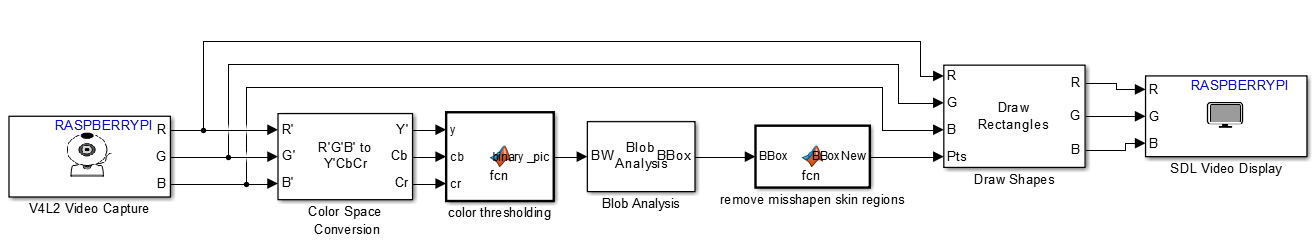
\includegraphics[width=14cm]{./img/simulink/Simulink_RaspberryPi.PNG} 
\caption{Simulink model - Run on Raspberry Pi}
\end{figure}


\end{document}
